\documentclass[a4paper]{article}
\usepackage{siunitx}

% Этот шаблон документа разработан в 2014 году
% Данилом Фёдоровых (danil@fedorovykh.ru) 
% для использования в курсе 
% <<Документы и презентации в \LaTeX>>, записанном НИУ ВШЭ
% для Coursera.org: http://coursera.org/course/latex .
% Исходная версия шаблона --- 
% https://www.writelatex.com/coursera/latex/5.3

% В этом документе преамбула

\usepackage{siunitx}
%%% Работа с русским языком
\usepackage{cmap}					% поиск в PDF
\usepackage{mathtext} 				% русские буквы в формулах
\usepackage[T2A]{fontenc}			% кодировка
\usepackage[utf8]{inputenc}			% кодировка исходного текста
\usepackage[english,russian]{babel}	% локализация и переносы
\usepackage{indentfirst}
\frenchspacing

\renewcommand{\epsilon}{\ensuremath{\varepsilon}}
\renewcommand{\phi}{\ensuremath{\varphi}}
\renewcommand{\kappa}{\ensuremath{\varkappa}}
\renewcommand{\le}{\ensuremath{\leqslant}}
\renewcommand{\leq}{\ensuremath{\leqslant}}
\renewcommand{\ge}{\ensuremath{\geqslant}}
\renewcommand{\geq}{\ensuremath{\geqslant}}
\renewcommand{\emptyset}{\varnothing}
\renewcommand{\Im}{\operatorname{Im}}
\renewcommand{\Re}{\operatorname{Re}}


%%% Дополнительная работа с математикой
\usepackage{amsmath,amsfonts,amssymb,amsthm,mathtools} % AMS
\usepackage{icomma} % "Умная" запятая: $0,2$ --- число, $0, 2$ --- перечисление

%% Номера формул
%\mathtoolsset{showonlyrefs=true} % Показывать номера только у тех формул, на которые есть \eqref{} в тексте.
%\usepackage{leqno} % Нумереация формул слева

%% Свои команды
\DeclareMathOperator{\sgn}{\mathop{sgn}}
\DeclareMathOperator{\sign}{\mathop{sign}}
\DeclareMathOperator*{\res}{\mathop{res}}
\DeclareMathOperator*{\tr}{\mathop{tr}}

%% Перенос знаков в формулах (по Львовскому)
\newcommand*{\hm}[1]{#1\nobreak\discretionary{}
{\hbox{$\mathsurround=0pt #1$}}{}}

%%% Работа с картинками
\usepackage{graphicx}  % Для вставки рисунков
\graphicspath{{figures/}}  % папки с картинками
\setlength\fboxsep{3pt} % Отступ рамки \fbox{} от рисунка
\setlength\fboxrule{1pt} % Толщина линий рамки \fbox{}
\usepackage{wrapfig} % Обтекание рисунков текстом

%%% Работа с таблицами
\usepackage{array,tabularx,tabulary,booktabs} % Дополнительная работа с таблицами
\usepackage{longtable}  % Длинные таблицы
\usepackage{multirow} % Слияние строк в таблице

%%% Теоремы
\theoremstyle{plain} % Это стиль по умолчанию, его можно не переопределять.
\newtheorem{theorem}{Теорема}
\newtheorem*{thm}{Теорема}
\newtheorem{prop}{Утверждение}
 
\theoremstyle{definition} % "Определение"
%\newtheorem{corollary}{Следствие}[theorem]
\newtheorem*{dfn}{Определение}
\newtheorem{problem}{Задача}
\newtheorem*{problem*}{Задача}

 
\theoremstyle{remark} % "Примечание"
\newtheorem*{sol}{Решение}
\newtheorem*{rem}{Замечание}

%%% Программирование
\usepackage{etoolbox} % логические операторы

%%% Страница
%\usepackage{extsizes} % Возможность сделать 14-й шрифт
%\usepackage{geometry} % Простой способ задавать поля
%	\geometry{top=25mm}
%	\geometry{bottom=35mm}
%	\geometry{left=35mm}
%	\geometry{right=20mm}
 
\usepackage{fancyhdr} % Колонтитулы
%	\pagestyle{fancy}
 %	\renewcommand{\headrulewidth}{0pt}  % Толщина линейки, отчеркивающей верхний колонтитул
	%\lfoot{Нижний левый}
	%\rfoot{Нижний правый}
	%\rhead{Верхний правый}
	%\chead{Верхний в центре}
	%\lhead{Верхний левый}
	%\cfoot{Нижний в центре} % По умолчанию здесь номер страницы

\usepackage{setspace} % Интерлиньяж
%\onehalfspacing % Интерлиньяж 1.5
%\doublespacing % Интерлиньяж 2
%\singlespacing % Интерлиньяж 1

\usepackage{lastpage} % Узнать, сколько всего страниц в документе.

\usepackage{soul} % Модификаторы начертания

\usepackage{hyperref}
%\usepackage[usenames,dvipsnames,svgnames,table,rgb]{xcolor}
\hypersetup{				% Гиперссылки
    unicode=true,           % русские буквы в раздела PDF
    pdftitle={Заголовок},   % Заголовок
    pdfauthor={Автор},      % Автор
    pdfsubject={Тема},      % Тема
    pdfcreator={Создатель}, % Создатель
    pdfproducer={Производитель}, % Производитель
    pdfkeywords={keyword1} {key2} {key3}, % Ключевые слова
    colorlinks=true,       	% false: ссылки в рамках; true: цветные ссылки
    linkcolor=red,          % внутренние ссылки
    citecolor=black,        % на библиографию
    filecolor=magenta,      % на файлы
    urlcolor=cyan           % на URL
}

\usepackage{csquotes} % Еще инструменты для ссылок

%\usepackage[style=apa,maxcitenames=2,backend=biber,sorting=nty]{biblatex}

\usepackage{multicol} % Несколько колонок

\usepackage{tikz} % Работа с графикой
\usepackage{pgfplots}
\usepackage{pgfplotstable}
%\usepackage{coloremoji}
\usepackage{floatrow}
\usepackage{subcaption}
\newcommand*{\N}{\mathbb{N}}
\newcommand*{\R}{\mathbb{R}}
\newcommand*{\K}{\mathbb{K}}
\newcommand*{\V}{\mathcal{V}}
\newcommand*{\A}{\mathcal{A}}
\newcommand*{\ii}{\mathbf{1}}
\newcommand*{\oo}{\mathbf{0}}
\newcommand*{\ba}{\mathbf{a}}
\newcommand*{\bb}{\mathbf{b}}
\newcommand*{\Q}{\mathbb{Q}}
\graphicspath{{figures/}}
%\usepackage{breqn}

\renewcommand\thesubfigure{\asbuk{subfigure}}
%\addbibresource{master.bib}

\usepackage{import}
\usepackage{pdfpages}
\usepackage{transparent}
\usepackage{xcolor}
\usepackage{xifthen}

%\newcommand{\incfig}[1]{%
%    \def\svgwidth{\columnwidth}
%    \import{./figures/}{#1.pdf_tex}
%}


\newcommand{\incfig}[2][1]{%
    \def\svgwidth{#1\columnwidth}
    \import{./figures/}{#2.pdf_tex}
}
\usepackage{titlesec}
%\titleformat{\section}{\normalfont\Large\bfseries}{}{0pt}{}
%----------------------STANDART:
%\titleformat{\chapter}[display]
%  {\normalfont\huge\bfseries}{\chaptertitlename\ \thechapter}{20pt}{\Huge}
%\titleformat{\section}{\normalfont\Large\bfseries}{\thesection}{1em}{}
%\titleformat{\subsection}
%  {\normalfont\large\bfseries}{\thesubsection}{1em}{}
%\titleformat{\subsubsection}
%  {\normalfont\normalsize\bfseries}{\thesubsubsection}{1em}{}
%\titleformat{\paragraph}[runin]
%  {\normalfont\normalsize\bfseries}{\theparagraph}{1em}{}
%\titleformat{\subparagraph}[runin]
%  {\normalfont\normalsize\bfseries}{\thesubparagraph}{1em}{}

\pdfsuppresswarningpagegroup=1
\pgfplotsset{compat=1.16}

\usepackage{xifthen}
\makeatother
%\def\@lecture{}%
%\newcommand{\lecture}[3]{
%    \ifthenelse{\isempty{#3}}{%
%        \def\@lecture{Неделя #1}%
%    }{%
%        \def\@lecture{Неделя #1: #3}%
%    }%
%    \section*{\@lecture}
%    \marginpar{\small\textsf{\mbox{#2}}}
%}
\makeatletter

%\newcommand{\lec}{\subsection{Лекция}}
%\newcommand{\sem}{\subsection{Семинар}}
%\newcommand{\hw}{\subsection{Домашняя работа}}
%\newcommand{\prob}[1]{\textbf{#1}}
%\renewcommand{\thesubsection}{}
%\renewcommand{\thesubsubsection}{}

%\setcounter{tocdepth}{1} % only parts,chapters,sections
%\titleformat{\subsection}{\normalfont\large\bfseries}{}{0em}{}
%\titleformat{\subsubsection}{\normalfont\normalsize\bfseries}{}{0em}{}

%\newcommand{\textover}[2]{\stackrel{\mathclap{\normalfont\mbox{#2}}}{#1}}

\author{Драчов Ярослав\\
Факультет общей и прикладной физики МФТИ}
\newcommand{\veq}{\mathrel{\rotatebox{90}{$=$}}}
%\newcommand{\teto}[1]{\stackrel{\mathclap{\normalfont\tiny\mbox{#1}}}{\to}}
%\renewcommand{\thesubsection}{\arabic{subsection}}

%%\setcounter{secnumdepth}{0}

\definecolor{tabblue}{RGB}{30, 119, 180}
\definecolor{taborange}{RGB}{255, 127, 15}
\definecolor{tabgreen}{RGB}{45, 160, 43}
\definecolor{tabred}{RGB}{214, 38, 40}
\definecolor{tabpurple}{RGB}{148, 103, 189}
\definecolor{tabbrown}{RGB}{140, 86, 76}
\definecolor{tabpink}{RGB}{227, 119, 193}
\definecolor{tabgray}{RGB}{127, 127, 127}
\definecolor{tabolive}{RGB}{188, 189, 33}
\definecolor{tabcyan}{RGB}{22, 190, 207}
\pgfplotscreateplotcyclelist{colorbrewer-tab}{
{tabblue},
{taborange},
{tabgreen},
{tabred},
{tabpurple},
{tabbrown},
{tabpink},
{tabgray},
{tabolive},
{tabcyan},
}
\usepackage{csvsimple}
\usepackage{extarrows}
%\renewcommand{\labelenumii}{\asbuk{enumii})}
%\renewcommand{\labelenumiv}{\Asbuk{enumiv}}
\newcommand{\prob}[1]{\subsubsection*{#1}}
\sisetup{output-decimal-marker = {,},separate-uncertainty = true,exponent-product = \cdot}

\usepackage{braket}
\usepackage{enumerate}
\usepackage{chngcntr}
%\counterwithin*{equation}{problem}
%\usepackage{bbold}

\newtheoremstyle{hiProb}% ⟨name ⟩ 
{3pt}% ⟨Space above ⟩1 
{3pt}% ⟨Space below ⟩1
{}% ⟨Body font ⟩
{}% ⟨Indent amount ⟩2
{\bfseries}% ⟨Theorem head font⟩
{.}% ⟨Punctuation after theorem head ⟩
{.5em}% ⟨Space after theorem head ⟩3
%{\thmname{#1} \thmnote{#3}}% ⟨Theorem head spec (can be left empty, meaning ‘normal’)⟩
{\thmnote{#3}}% ⟨Theorem head spec (can be left empty, meaning ‘normal’)⟩
\theoremstyle{hiProb} % "Определение"
%\newtheorem{hiProb}{Задача}
\newtheorem{hiProb}{}
\usepackage{mmacells}
\newcommand{\textover}[2]{\stackrel{\mathclap{\normalfont\scriptsize\mbox{#2}}}{#1}}
\usepackage{units}
\usepackage[math]{cellspace}%
\setlength\cellspacetoplimit{2pt}
\setlength\cellspacebottomlimit{2pt}

\title{Лабораторная работа №1.1\\  <<Экспериментальная проверка уравнения Эйнштейна для фотоэффекта>>}
\author{Драчов Ярослав \\ \Факультет общей и прикладной физики МФТИ}
\begin{document}
\maketitle
\section{Введение}
В данной лабораторной работе будет происследована зависимость
фототока от величины задерживающего потенциала и частоты
падающего излучения, что позволит вычислить величину постоянной
Планка.
\section{Теоретическое введение}
\emph{Фотоэффект} -- испускание электронов фотокатодом, облучаемым
светом  --- хорошо объясняется фотонной теорией света: фотон
с энергией $\hbar \omega$ выбивает электрон из поверхности
металла и сообщает электрону кинетическую энергию.

Энергетический баланс этого взаимодействия описывается уравнением:
\begin{equation}
	\hbar \omega = W + E_{\text{max}},
	\label{eq:1}
\end{equation}
где $W$ --- работа выхода электрона из катода, $E_{\text{maax}}$ ---
максимальная кинетическая энергия электрона после выхода из
фотокатода. Реально энергетический спектр вылетевших из фотокатода
электронов непрерывный --- он простирается от нуля до
$E_{\text{max}}$.

Для измерения энергии вылетевших фотоэлектронов вблизи фотокатода
обычно располагается второй электрод (анод), на который подаётся
задерживающий ($V<0$) или ускоряющий $(V>0)$ потенциал. При
достаточно больших ускоряющих напряжениях фототок достигает
насыщения (рис.~\ref{fig:1}):
\begin{figure}[h]
	\centering
	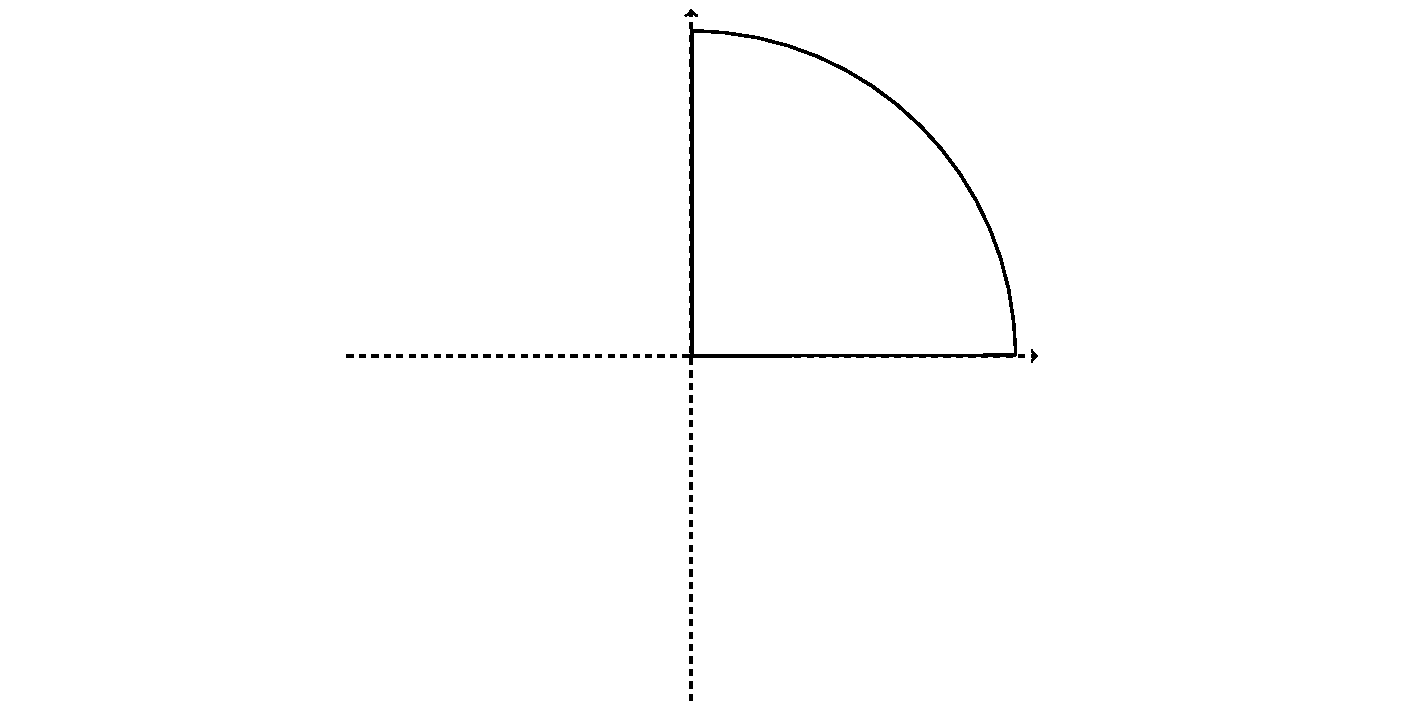
\includegraphics[width=0.4\textwidth]{1.pdf}
	\caption{Зависимость фототока от напряжения на аноде}
	\label{fig:1}
\end{figure}
все испущенные электроны попадают на анод. При задерживающих
потенциалах на анод попадают лишь электроны, обладающие достаточно
большой кинетической энергией, в то время как медленно
движущиеся электроны заворачиваются полем и возвращаются на
катод. При некотором значении $V=-V_0$ (потенциал запирания)
даже наиболее быстрые фотоэлектроны не могут достичь анода.

Максимальная кинетическая энергия $E_{\text{max}}$ электронов
связана с запирающим потенциалом $V_0$ очевидным соотношением:
$E_{\text{max}}=e V_0 $ . Поставляя это соотношение в равенство (\ref{eq:1}), мы получаем уравнение Эйнштейна для фотоэффекта:
\begin{equation}
	e V_0= \hbar \omega -W
	\label{eq:2}
.\end{equation}

Чтобы определить величину запирающего напряжения, нам надо
правильно экстраполировать получаемую токовую зависимость к нулю,
т.\:е. определить, какова функциональная зависимость $I(V)$.
Расчёт для простейшей геометрии --- плоский катод, освещаемый светом,
и параллельный ему анод --- приводит к зависимости
\begin{equation}
	\sqrt{I} \propto (V_0-V)
	\label{eq:3}
.\end{equation}
то есть, корень квадратный из фототока линейно зависит от
запирающего напряжения.

Для экспериментальной проверки уравнения Эйнштейна по графикам
$\sqrt{I} =f(V)$ определяются  потенциалы запирания $V_0$ при
разных частотах и строится зависимость $V_0(w)$, которая, как
следует из (\ref{eq:2}), должна иметь вид
\begin{equation}
	V_0(\omega)=\frac{\hbar \omega-W}{e}
	\label{eq:4}
.\end{equation}
Потенциал запирания $V_0$ для всякого данного катода линейно
зависит от частоты света $\omega$. По наклону прямой на графике
$V_0(\omega)$(рис.~\ref{fig:2})
\begin{figure}[h]
	\centering
	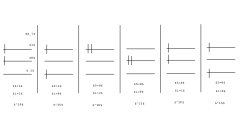
\includegraphics[width=0.4\textwidth]{2}
	\caption{Зависимость потенциала запирания от частоты}
	\label{fig:2}
\end{figure}
можно определить постоянную Планка:
\begin{equation}
	\frac{dV_0}{d\omega}=\frac{\hbar}{e}
	\label{eq:5}
.\end{equation}
Как показывает формула (\ref{eq:5}), угол наклона прямой $V_0(\omega)$
не зависит от рода вещества, из которого изготовлен фотокатод. От
рода вещества, однако, зависит величина фототока, работа выхода
$W$ и форма кривой $I(V)$ (рис.~\ref{fig:1}). Всё это определяет
выбор пригодных для опыта катодов.

В особенноости важноо, чтобы кривая $I(V)$ достаточноо круто
подходила к нулю.
\section{Экспериментальная установка}
Схема установки приведена на рис.~\ref{fig:3}.
\begin{figure}[h]
	\centering
	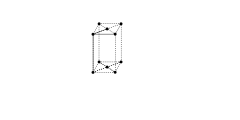
\includegraphics[width=0.6\textwidth]{3}
	\caption{Схема экспериментальной установки}
	\label{fig:3}
\end{figure}
Свет от источника $S$ (электрическая лампа накаливания) с помощью
конденсора фокусируется на входную щель призменного монохроматора
УМ-2, выделяющего узкий спектральный интервал, и попадает на катод
фотоэлемента Ф-25. В качестве катода в данноом фотоэлементе используется
$\mathrm{Na_2\,K\, Sb(Cs)}$ покрытие. На рис.~\ref{fig:4}
\begin{figure}[h]
	\centering
	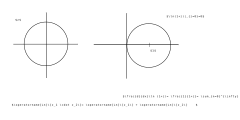
\includegraphics[width=0.4\textwidth]{4}
	\caption{Чувствительность фотокатода (а) и характеристика
	излучения лампы накаливания (б)}
	\label{fig:4}
\end{figure}
показаны относительная спектральная чувствительность фотокатода
(6а) и спектральная характеристика излучения лампы накаливания
(6б).

Призменный монохроматр-спектрометр УМ-2 (универсальный монохроматор)
предназначен для спектральных исследований в диапазоне от 0,38 до
1,00 мкм. Основные элементы монохроматора представлены на рис.~\ref{fig:5}.
\begin{figure}[h]
	\centering
	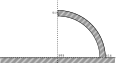
\includegraphics[width=0.4\textwidth]{5}
	\caption{Схема монохроматора}
	\label{fig:5}
\end{figure}
\begin{enumerate}
	\item Входная щель 1б снабжённая микрометрическим винтом
		9, который позволяет открывать щель на нужную
		ширину (в диапазоне 0,01--4~мм).
	\item Коллиматорный объектив 2, снабжённый микрометрическим
		винтом 8. Винт позволяет смещать объектив
		относительно щели при фокусировке спектральных
		линий различных цветов.
	\item Сложная спетральная призма 3, установленная на
		поворотноом столике 6. Призма 3 состоит из трёх
		склеенных призм $\Pi_1,\, \Pi_2$ и $\Pi_3$.
		Первые две призмы с преломляющими углами $30^\circ$
		изготовлены из тяжёлого флинта, обладающего большой
		дисперсией. Промежуточная призма  $\Pi_3$ сделана
		из крона. Лучи отражаются от её гипотенузой
		грани и поворачиваются на $90^\circ$. Благодаря
		такому устройству дисперсия призм $\Pi_1$ и $\Pi_2$
		складываются.
	 \item Поворотный столик 6, вращающийся вокруг вертикальной
		 оси при помощи микрометрического винта с
		 отсчётным барабаном. На барабан нанесена винтовая
		 дорожка с градусными делениями. Вдоль дорожки
		 скользит указатель барабана. При вращении
		 барабана призма поворачивается, и в центре поля
		 зрения появляются различные участки спектра.
	\item Зрительная труба, состоящая из объектива 4
		 и блока окуляра 5. Объектив даёт изображение
		 входной щели 1 различных цветов в своей фокальной
		 плоскости. В этой же плоскости расположено
		 острие указателя 10. Изображение щели
		 рассматривается через окуляр 5.

		 Тумблеры, расположенные на основании спектрометра,
		 позволяют включать лампачки осветителей шкал и
		 указателя спектральных линий. Яркость освещения
		 указателя регулируется реостатом.

		 В случае необходимости, освободив винт 12, блок
		 окуляра можно заменить входной щелью фотоэлемента,
		 пропускающей всего одну из линий спектра на
		 фотоэлемент.
	\item Массивный корпус 11, предохраняющий прибор от
		повреждений и загрязнений.
	\item Оптическая скамья, на которой могут перермещаться
		рейтеры с источником света Л и конденсатором К,
		служащим для концентрации света на входной щели.
		Входная щель спектрометра, конденсор и источник
		должны быть на одной высоте.
		Проходящий через входую щель световой пучок хорошо
		заполняет конденсор и призму, если выполнено
		соотношение $D_k /b= D_2 /f_2= 1 /6$, где $D_k$ ---
		диаметр конденсора, $b$ --- расстояние от
		конденсора до входной щели, $D_2$ и $f_2$ ---
		диаметр и фокусное расстояние коллиматорного
		объектива 2.

		Изображение удобно наблюдать на белом колпачке
		с крестиком (таким колпачком прикрывают щель при
		юстировке системы).
	\item Пульт управления (на рис.~\ref{fig:3} не показан),
		служащий для питания лампы накаливания и
		осветительной системы спектрометра.
\end{enumerate}
\section{Ход работы}
Используя окуляр, прооградуируем барабан монохроматора по спектру
неоновой лампы (таблица \ref{tab:1})
\begin{table}[h]
\begin{tabular}{|l|l|}
\hline
$\lambda,$ \AA & $\alpha, \; ^\circ$ \\ \hline
6507 & 2786 \\ \hline
6402 & 2742 \\ \hline
6334 & 2716 \\ \hline
6267 & 2684 \\ \hline
6163 & 2644 \\ \hline
6096 & 2616 \\ \hline
6030 & 2584 \\ \hline
5976 & 2560 \\ \hline
5882 & 2514 \\ \hline
5401 & 2236 \\ \hline
\end{tabular}
\caption{Градуировка барабана монохроматора по спектру неоновой
лампы}
\label{tab:1}
\end{table}
Пользуясь полученной градуировкой снимем зависимость запирающего
напряжения от частоты излучения падающего света (таблица \ref{tab:2}).
\begin{table}[h]
\begin{tabular}{|l|l|}
\hline
$\omega,\; 10^{15}\cdot \text{с}^{-1}$&$U_{\text{З}},$ В\\ \hline
2,897 & 0,37 \\ \hline
2,976 & 0,42 \\ \hline
3,058 & 0,47 \\ \hline
3,126 & 0,51 \\ \hline
3,154 & 0,52 \\ \hline
3,205 & 0,55 \\ \hline
3,490 & 0,71 \\ \hline
\end{tabular}
\caption{Зависимость запирающего напряжения от частоты излучения
падающего света}
\label{tab:2}
\end{table}
Построим график данной зависимости (рис.~\ref{fig:6}).
\begin{figure}[h]
	\centering
	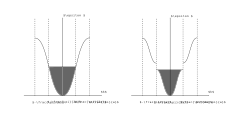
\includegraphics[width=0.8\textwidth]{6}
	\caption{Зависимость запирающего напряжения от частоты
	излучения падающего света}
	\label{fig:6}
\end{figure}
По графику определим постоянную Планка:
\begin{equation}
	\frac{dV_0}{d\omega}=(577\pm 7)\cdot 10^{-18} \text{В}\cdot
	\text{с}=
\frac{\hbar}{e}
.\end{equation}
Откуда
\begin{equation}
\hbar=(0,921\pm 0,011)
	\cdot 10^{-34} \text{Дж}\cdot \text{с}
.\end{equation}
Табличное же значение постоянной Планка: $\hbar\approx 1,054 \cdot 10^{-34}
 \text{Дж}\cdot \text{с}$.

По этому же графику можно найти красную границу спектра:
\begin{equation}
	\omega_{\text{к}}=(2,25 \pm 0,04)\cdot 10^{15} \text{с}^{-1}\quad
	\implies \quad \lambda_{\text{к}}=\frac{2 \pi c}{\omega
	_{\text{к}}}=(837 \pm 16) \cdot 10^1 \text{\AA}
,\end{equation}
и работу выхода:
\begin{equation}
	W=\hbar \omega_{\text{к}}=1,30\pm 0,03 \text{эВ}
.\end{equation}
Для длины волны $\lambda=6507 \text{ \AA}$ также измерим зависимость
фототока от напряжения на аноде (таблица \ref{tab:3}).
\begin{table}[h]
\begin{tabular}{|l|l|}
\hline
$U_{\text{А}}$, В      & $U_{\text{Ф}}$,  В     \\ \hline
0,019  & 0,240  \\ \hline
-0,040 & 0,193  \\ \hline
-0,077 & 0,164  \\ \hline
-0,118 & 0,132  \\ \hline
-0,150 & 0,109  \\ \hline
-0,178 & 0,0883 \\ \hline
-0,216 & 0,0626 \\ \hline
-0,251 & 0,0430 \\ \hline
-0,283 & 0,0290 \\ \hline
-0,314 & 0,0185 \\ \hline
-0,354 & 0,0095 \\ \hline
-0,369 & 0,0075 \\ \hline
\end{tabular}
\caption{Зависимость фототока от напряжения на аноде}
\label{tab:3}
\end{table} 
По данной зависимости построим график $\sqrt{I} =f(V)$ (рис.~\ref{fig:7}).
\begin{figure}[h]
	\centering
	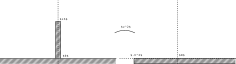
\includegraphics[width=0.8\textwidth]{7}
	\caption{Зависимость фототока от напряжения на аноде}
	\label{fig:7}
\end{figure}
Если предположить что данная зависимость должна быть линейной,
то значение запирающего напряжения будет отличаться от того, что
мы наблюдаем на эксперименте и будет численно равно $0,396\pm 0,015$
В.
\section{Выводы}
В ходе выполнения работы мы пронаблюдали явление фотоэффекта и
с помощью уравнения Эйнштейна измерили постоянную Планка, а
также оценили красную границу спектра и работу выхода для
нашей установки. Причина небольшого несовпадения полученного
значения постоянной Планка с её табличным значением кроется в
неточности использованной в данной работе методики измерений.
Возможно, мы бы наблюдали полное совпадение экспериментальных
данных с табличными в пределах погрешности, если бы находили
запирающее напряжение по ВАХ для каждой отдельной частоты, т.\:к.
мы убедились, что данный факт действительно влияет на
получаемые результаты.
\definecolor{tabblue}{RGB}{30, 119, 180}
\definecolor{taborange}{RGB}{255, 127, 15}
\definecolor{tabgreen}{RGB}{45, 160, 43}
\definecolor{tabred}{RGB}{214, 38, 40}
\definecolor{tabpurple}{RGB}{148, 103, 189}
\definecolor{tabbrown}{RGB}{140, 86, 76}
\definecolor{tabpink}{RGB}{227, 119, 193}
\definecolor{tabgray}{RGB}{127, 127, 127}
\definecolor{tabolive}{RGB}{188, 189, 33}
\definecolor{tabcyan}{RGB}{22, 190, 207}
\pgfplotscreateplotcyclelist{colorbrewer-tab}{
{tabblue},
{taborange},
{tabgreen},
{tabred},
{tabpurple},
{tabbrown},
{tabpink},
{tabgray},
{tabolive},
{tabcyan},
}
\begin{tikzpicture} \begin{axis}
[cycle list name=colorbrewer-tab,
title=Какой-то график,
minor x tick num=0,
minor y tick num=1,
xlabel={$\sum_{n=1}^{\infty} a_n z^n$, см},
ylabel={$e^t$, c},
grid=both,
line width=0.6pt,
tick style={line width=0.6pt},
grid style={line width=0.6pt},
]
\addplot+ [
only marks, error bars/.cd,
error bar style={line width=0.6pt},
error mark options={rotate=90,line width=0.6pt},
            x dir=both, x explicit,
            y dir=both, y explicit,
    ] table [x=a, x error=b, y=c, y error=d %, col sep= comma
]{trash/dataset.csv};
\addplot+ [line width =1pt,domain=-0:0.4,samples=201] {0.5 - x};
\end{axis}
\end{tikzpicture}
\num{15.(3)e-4}
\end{document}
